\question \textbf{Prehistoric States} \\*
A prehistoric civilization survives by hunting game in the forests near 
their home. At the beginning of the hunting season, all the young men 
go out to the forest. After the first day, those who have a kill, 
which happens with probability 1/2, return home. Everyone who has been 
out for two days, even if without a kill, returns home for rest. And 
everyone who goes home goes back out the next day.
\begin{enumerate}
\item
What are the states in this scenario? Draw a Markov chain.
\begin{solution}[4cm]
We need distinct states for at home, day 1, and day 2, because the 
probabilities of changing depend on these, and only these. Letting 0, 
1, and 2 represent these states, we have

\begin{center}
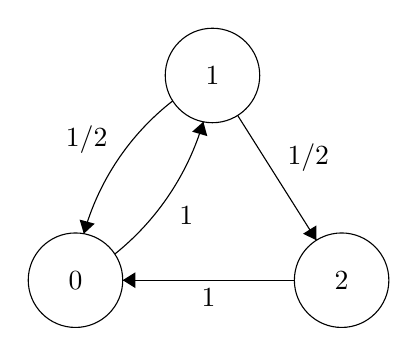
\begin{tikzpicture}[scale=0.2]
\tikzstyle{every node}+=[inner sep=0pt]
\draw [black] (42,-21.2) circle (3);
\draw (42,-21.2) node {$1$};
\draw [black] (50.2,-34.2) circle (3);
\draw (50.2,-34.2) node {$2$};
\draw [black] (33.3,-34.2) circle (3);
\draw (33.3,-34.2) node {$0$};
\draw [black] (43.6,-23.74) -- (48.6,-31.66);
\fill [black] (48.6,-31.66) -- (48.6,-30.72) -- (47.75,-31.25);
\draw (46.73,-26.4) node [right] {$1/2$};
\draw [black] (33.829,-31.251) arc (164.5081:127.90859:16.168);
\fill [black] (33.83,-31.25) -- (34.52,-30.61) -- (33.56,-30.35);
\draw (35.36,-25.24) node [left] {$1/2$};
\draw [black] (41.419,-24.139) arc (-16.28943:-51.29388:16.81);
\fill [black] (41.42,-24.14) -- (40.71,-24.77) -- (41.67,-25.05);
\draw (39.86,-30.11) node [right] {$1$};
\draw [black] (47.2,-34.2) -- (36.3,-34.2);
\fill [black] (36.3,-34.2) -- (37.1,-34.7) -- (37.1,-33.7);
\draw (41.75,-34.7) node [below] {$1$};
\end{tikzpicture}
\end{center}
\end{solution}

\newpage
\item
What is the transition matrix? The  initial vector?
\begin{solution}[4cm]
$ P = \begin{bmatrix}
0 & 1 & 0 \\
\frac{1}{2} & 0 & \frac{1}{2} \\
1 & 0 & 0
\end{bmatrix} \\
\pi = \begin{bmatrix} 1 & 0 & 0 \end{bmatrix}$ because everyone starts 
at home.
\end{solution}

\item
Is this Markov chain reducible? Is it periodic?
\begin{solution}[2cm]
This chain is irreducible, because there is a path from any node to any 
other. It is aperiodic (I THINK), because, for instance, weight that 
starts at node 0 can “return” in either 2 or 3 iterations.
\end{solution}

\item
What is the invariant vector?
\begin{solution}[4cm]
$\begin{bmatrix} \pi_1 & \pi_2 & \pi_3 \end{bmatrix}
= \pi = \pi P = 
\begin{bmatrix} \pi_1 & \pi_2 & \pi_3 \end{bmatrix}
\begin{bmatrix}
0 & 1 & 0 \\ \frac{1}{2} & 0 & \frac{1}{2} \\ 1 & 0 & 0 
\end{bmatrix} = 
\begin{bmatrix} \frac{\pi_2}{2} + \pi_3 & p_1 & \frac{\pi_2}{2} \end{bmatrix}
$
Thus
$ \pi = \begin{bmatrix} \pi_1 & \pi_2 & \pi_3 \end{bmatrix}
= \begin{bmatrix} \frac{2}{5} & \frac{2}{5} & \frac{1}{5} \end{bmatrix}
$
\end{solution}

\item
What are the distributions after one week?
\begin{solution}[6cm]
$ 
P^2 = 
\begin{bmatrix}
\frac{1}{2} & 0 & \frac{1}{2} \\
\frac{1}{2} & \frac{1}{2} & 0 \\
0 & 1 & 0
\end{bmatrix}
p^4 = 
\begin{bmatrix}
\frac{1}{4} & \frac{1}{2} & \frac{1}{4} \\
\frac{1}{2} & \frac{1}{4} & \frac{1}{4} \\
\frac{1}{2} & \frac{1}{2} & 0\end{bmatrix} 
P^6 = 
\begin{bmatrix}
\frac{3}{8} & \frac{1}{2} & \frac{1}{8} \\
\frac{3}{8} & \frac{3}{8} & \frac{1}{4} \\
\frac{1}{2} & \frac{1}{4} & \frac{1}{4}
\end{bmatrix} 
P^7 = 
\begin{bmatrix}
\frac{3}{8} & \frac{3}{8} & \frac{1}{4} \\
\frac{7}{16} & \frac{3}{8} & \frac{3}{16} \\
\frac{3}{8} & \frac{1}{2} & \frac{1}{8}
\end{bmatrix} \\ $
Thus we have $\pi p^7 = \begin{bmatrix} 1 & 0 & 0 \end{bmatrix} 
\begin{bmatrix} 
\frac{3}{8} & \frac{3}{8} & \frac{1}{4} \\
\frac{7}{16} & \frac{3}{8} & \frac{3}{16} \\
\frac{3}{8} & \frac{1}{2} & \frac{1}{8}
\end{bmatrix} = 
\begin{bmatrix} \frac{3}{8} & \frac{3}{8} & \frac{1}{4} \end{bmatrix}$
\end{solution}

\item
What is the expected length of hunting trip?
\begin{solution}[2cm]
Pr[takes 2 days] = $\frac{1}{2}$. Pr[takes 3 days] = $\frac{1}{2}$.
Expected Value = $2(\frac{1}{2}) + 3(\frac{1}{2}) = 2.5$
\end{solution}
\end{enumerate}